\documentclass[runningheads]{llncs}
\usepackage{amssymb}
\setcounter{tocdepth}{3}
\usepackage{graphicx,epsfig}
\usepackage{algorithmic}
\usepackage{listings}
\usepackage{rotating}
\usepackage{subfig}

%%%%

\usepackage{color}
\usepackage{alltt}
\usepackage{verbatim}
\usepackage{url}
\usepackage[latin1]{inputenc}
%\usepackage[spanish]{babel}

%%

\usepackage{url}
%\urldef{\mailsa}\path|pgarcia@atc.ugr.es|

\urldef{\mailsa}\path|pgarcia@atc.ugr.es|

\newcommand{\keywords}[1]{\par\addvspace\baselineskip
\noindent\keywordname\enspace\ignorespaces#1}

\lstset{
basicstyle=\ttfamily \scriptsize,
language=c++,
frame=single,
stringstyle=\ttfamily,
showstringspaces=false
}

\renewcommand{\textfraction}{0}
\renewcommand{\topfraction}{1}
\renewcommand{\bottomfraction}{1}
\renewcommand{\floatpagefraction}{0.9}

\begin{document}

\mainmatter  % start of an individual contribution



% first the title is needed
\title{Desarrollo de servicios para una Arquitectura Orientada a Servicios para Algoritmos Evolutivos \thanks{Este trabajo ha sido desarrollado bajo los proyectos EvOrq (TIC-3903), CEI BioTIC GENIL (CEB09-0010), MICINN CEI Program (PYR-2010-13) and FPU research grant AP2009-2942 .
}}


% a short form should be given in case it is too long for the running head
\titlerunning{Desarrollo de servicios para una Arquitectura Orientada a Servicios para Algoritmos Evolutivos}
%\author{No author given}
\author{P. Garc\'ia-S\'anchez\inst{1}, A. E. Eiben\inst{2}, E. Haasdijk\inst{2}, B. Weel\inst{2} and J.J. Merelo\inst{1}}

%

\authorrunning{P. Garc\'ia-S\'anchez et al.}
%\authorrunning{Anonymous.}
% (feature abused for this document to repeat the title also on left hand pages)
% the affiliations are given next; don't give your e-mail address
% unless you accept that it will be published

\institute{Dept. of Computer Architecture and Technology, University of Granada, Spain \and Dept. of Computer Science, Vrije Universiteit Amsterdam, The Netherlands
\mailsa}
%\institute{No institute given
%\mailsa}




%\toctitle{BLABLABLA}

%\tocauthor{Authors' Instructions}
\maketitle


\begin{abstract}
We investigate on-line on-board evolution of robot controllers based
on the so-called hybrid approach (island-based). Inherently to this approach each
robot hosts a population (island) of evolving controllers and
exchanges controllers with other robots at certain times. We compare
different exchange (migration) policies in order to optimize this
evolutionary system and compare the best hybrid setup with the
encapsulated and distributed alternatives. We conclude that adding a difference-based migrant
 selection scheme increases the performance.
%Not too clear now. You don't define hybrid , and what I understand
%here is that you optimize something and you compare it with something
%else, but it's not clear what conclusion you obtain from the
%optimization and why do you compare it. Is it better? Worse? - JJ
%Pablo: added "(island-based)" and conclusions in the abstract
 
%This work presents the results obtained from comparing several migration policies that tries to optimize in a noisy fitness environment: the on-line, on-board and hybrid evolutionary robotics problem. Three different migration policies have been studied (the most different migrant, random migrant and best migrant) and two replacement mechanisms: the migrant replaces the worst, or the migrant replaces the worst after being evaluated only if is better. Experiments with 4, 16 and 36 robots were conduced, with two different topologies (ring and panmictic) and also a comparison with other evolutionary robotics algorithms were performed. Results show that the replacement mechanism has more influence than the migration policy or topology, and it also affects the tuning of the algorithm parameters.

% You should conclude something about the
            % "multiculturality" of the algorithm and explain results
            % via diversity - JJ

\end{abstract}

\section{Introduction}
\noindent Service Oriented Architecture (SOA) \cite{PAPAZOGLOU} se está convirtiendo en un importante TREND en el desarrollo de software. Este paradigma permite la organización y distribución utilizando el concepto de {\em servicio}. Un servicio es la interacción mostrada en la figura \ref{SOADIAGRAM}. El {\em proveedor de servicio} publica {\em descripciones de servicio} (o interfaces) en el {\em registro de servicios}, para que los {\em consumidores de servicio} puedan encontrarlo y enlazarse con los proveedores de servicio para usarlo.

SOA permite independencia en el lenguaje de programación y los mecanismos de distribución, centrándose en la extensión e integración fáciles, pero cuenta con las siguientes restricciones:

\begin{itemize}
\item Los servicios deben ser funciones de entrada/salida.
\item Los servicios no deben tener estado (es decir, no usar variables globales).
\item El orden de ejecución de los servicios no es fijo.
\item Los servicios deben ser diseñados tan abstractos como sea posible.
\end{itemize}

La computación distribuida ofrece la posibilidad de utilizar las ventajas del procesamiento paralelo y así conseguir un mayor poder de cómputo \cite{OPENSCIENCEGRID}.
SOA también puede aplicarse a este área, utilizando plataformas basadas en Web Services \cite{PAPAZOGLOU}, o nuevos estándars para este paradgima, como OSGi (Open Services Gateway Initiative) \cite{OSGI}.

OSGi permite construir sistemas software de calidad considerando un alto nivel de modularidad. Aparte de los beneficios que los paradigmas clásicos de modularización ofrecen (como el modelado orientado a objetos) y las mejoras en testeo, reusabilidad, disponibilidad y mantenibilidad, es necesario explorar otras técnicas, como el desarrollo basado en plug-ins o el diseño SOA. Este tipo de desarrollo simplifica aspectos como la complejidad, personalización, configuración, y coste del desarrollo. En el campo de las heurísticas de optimización los beneficios the usar este tipo de desarrollo tienen lugar en el desarrollo de algorithmos, evaluación experimental y combinación de diferentes paradigmas de optimización \cite{PLUGINS}.

 \begin{figure}[ht] 
\begin{center} 
 % \epsfig{file=soaDiagram.eps,width=7.5cm} 
\includegraphics[scale=1]{images/soaDiagram.eps}
\end{center} 
\caption{Esquema de interacción de servicios. El proveedor de servicios publica una descripción de servicio que es utilizada por el consumidor de servicios para encontrar y usar servicios.} 
\label{SOADIAGRAM} 
\end{figure} 

En nuestro trabajo anterior \cite{OSGILIATH} presentamos una Arquitectura Orientada a Servicios para Algoritmos Evolutivos (SOA-EA), junto con guías y pasos para migrar del desarrollo tradicional de Algoritmos Evolutivos (AEs) a SOA. También presentó una implementación específica, llamada OSGiLiath ({\em OSGi Laboratory for Implementation and Testing of Heuristics}): un entorno para el desarrollo de algoritmos distribuidos extensible con una arquitectura basada en plug-ins y basada en una especificación software ampliamente aceptada (OSGi). En este trabajo presentamos el desarrollo completo de un servicio utilizando la tecnología específica, en lugar del diseño abstracto presentado en nuestro anterior trabajo.

El resto del trabajo se estructura como sigue: después del estado del arte, presentamos los principios de diseño para crear servicios para Computación Evolutiva (CE) (Sección \ref{sec:design}). A continuación, se explica la tecnología de implementación OSGi en la Sección \ref{sec:technology}, utilizada para construir nuestro framework (descrito en la Sección \ref{sec:osgiliath}). Después, los pasos para crear servicios dentro de este framework se presentan (Sección \ref{sec:development}). Finalmente se presentan las conclusiones y trabajo futuro (Sección \ref{sec:conclusions}).



\section{Estado del arte}
\label{sec:soa}

Aunque SOA se usa ampliamente en el desarrollo de software no está muy aceptada en la comunidad de las metaheurísticas. La mayoría de los frameworks tienen carencia de la baja generalidad, ya que están enfocados en un campo específico, como EasyLocal++ \cite{EASYLOCAL}(centrado en Búsqueda Local) o SIGMA \cite{SIGMA} (en el campo de optimización de sistemas de soporte  a la decisión). Otro problema común es que suelen ser simplemente librerías o múdulos Perl \cite{PERL}, no tienen GUIs o son muy complicados de instalar y requieren muchas destrezas de programación. Otro problema puede ser la pérdida de confort a la hora de programar, por ejemplo, C tiene una sintaxis más complicada que otros lenguajes.

Entre la gran cantidad de herramientas software que existen, queremos centrarnos en los frameworks de algoritmos distribuídos más aceptados. ECJ \cite{ECJ}, Evolutionary Computation in Java, es un conjunto de clases Java que pueden ser extendidas e incluyen varios módulos de comunicación. MALLBA \cite{MALLBA} se basa en esqueletos software con una interfaz común pública. Cada esqueleto implementa una técnica de resolución para optimizaciónen el campo de optimización exacta, heurística o híbrida. Proporciona capacidades de distribución utilizando MPI. Sin embargo estos dos frameworks no se basan en el desarrollo orientado a plug-ins, por lo que no pueden tomar las ventajas de características como gestión del ciclo de vida, versionado o enlazado dinámico de servicios, como propone OSGi.

Otra plataforma importante es DREAM \cite{DREAM}, un framework open source para Algoritmos Evolutivos basado en Java que define un modelo de isla y usa el protocolo Gossip y sockets TCP/IP para comunicación. Puede desplegarse en plataformas P2P y está dividido en cinco capas. Cada capa proporciona una interfaz de usuario y diferentesniveles de interacción y abstracción, pero añadir nuevas funcionalidades no es tan fácil, debido al hecho de que el sistema debe pararse antes de añadir nuevos módulos y la implementación de interfaces debe estar definida en el código fuente, por lo que necesita compilarse con cada elemento a añadir (como en ECJ). OSGi permite añadir nuevas funcionalidades sólamente compilando las nuevas características y no ya las existentes.

Among this great number of software tools we want to focus in the most widely accepted distributed algorithms frameworks. ECJ \cite{ECJ}, Evolutionary Computation in Java, is a set of Java classes that can be extended and includes several communication modules. MALLBA \cite{MALLBA} is based in software skelletons with a common and public interface. Every skeleton implements a resolution technique for optimization in the fields of exact, heuristic or hybrid optimization. It provides LAN and WAN capacity distribution with MPI . However, this both frameworks are not based in the plug-in development, so they can not take advantage of features like the life-cycle management, versioning, or dynamic service binding, as OSGi proposes.

Los autores de MALLBA están trabajando ahora en el framework jMetal \cite{JMETAL}, un nuevo framework basado en Java, pero sin posibilidad de distribución y mayormente centrado en optimización Multi-Objetivo.

ParadiseEO \cite{PARADISEO} permite el diseño de AEs y Búsqueda Local con hibridación, proporcionando una gran variedad de operadores y funciones de evaluación. También implementa los modelos paralelos y distribuídos más comunes, y está basado en librerías estándar como MPI, PVM y Pthreads. Sin embargo, cuenta con los mismos problemas que los frameworks anteriores, no cuenta con gestión del ciclo de vida, ni programación orientada a servicios. GAlib \cite{GALIB} es muy similar y comparte las mismas características y problemas. 

En el campo de los frameworks basados en plug-ins, HeuristicLab \cite{HEURISTICLAB} es el ejemplo más avanzado. Permite además programación distribuída utilizando Servicios Web y una base de datos centralizada, pero no usa su propio diseño de plug-ins para la comunicación distribuída.


METCO  \cite{METCO} cuenta con los mismos problemas que los frameworks anteriores, no utiliza un sistema de plug-ins estándar ni SOA, pero permite la implementación de interfaces existentes y configurar sus funcionalidades. 

Finalmente, el único framework orientado a servicios para optimización es GridUFO \cite{GRIDUFO}, pero sólo permite la modificación de la función objetivo y añadir nuevos algoritmos, sin poder combinar servicios existentes.

Los frameworks anteriores han sido diseñados para ser extendibles y re-usables, pero sin tener en cuenta las restricciones de SOA para lograr más independencia y mejoras en el desarrollo.

\section{Algorithms and Experimental Setup}

We carried out our experiments with e-puck like robots simulated in the RoboRobo simulator\footnote{\url{http://www.lri.fr/~bredeche/roborobo/}}. The robot is controlled by an artificial neural net with 9 inputs (corresponding to the robot's distance sensors and a bias node), 2 outputs (wheel speeds). Genetically, this was represented as a vector coding the network's 18 weights. 
All algorithms were evaluated using the {\em Fast Forward} task and next fitness function: 
\vspace{-7pt}
\begin{equation}
\label{eq:fastfwd}
f = \sum_{t=0}^{\tau} (v_{t} \cdot (1 - v_{r}) )
\end{equation}
\vspace{-2pt} 

\noindent where $v_{t}$ and $v_{r}$ are the translational and the rotational speed, respectively. $v_t$ is normalised between $-1$ (full speed reverse) and $1$ (full speed forward), $v_r$ between $0$ (movement in a straight line) and $1$ (maximum rotation). Whenever a robot touches an obstacle, $v_t = 0$, so the fitness increment during collisions is 0. There is more information about this function in \cite{HUIJSMAN11}. This fitness is noisy: a controller configuration can produce different fitness values depending on the robot's position in the arena when evaluation starts. 
The robots are placed in a small maze-like arena
(Fig. \ref{fig:arena}). % You can eliminate this figure also for
                        % saving space. - JJ
                        % Pablo: reduced white that surrounded the figure.
To ensure a fair comparison across different numbers of robots, each robot is placed in a separate instance of the arena to avoid physical interaction between robots. Robots can communicate across arenas instances.

In our experiments, we compare three algorithms:

{\bf Encapsulated evolutionary algorithm}
The encapsulated algorithm we use is the $\mu+1$ on-line algorithm presented in \cite{Haasdijk2010On-line-evoluti}. Here, each robot runs a stand-alone evolutionary algorithm with a local population of $\mu$ individuals. In each cycle, one new solution (controller) is created and evaluated. This solution replaces the worst individual of the population if it has higher fitness. To combat the effects of noisy evaluations, an existing solution can be re-evaluated, instead of generating and testing a new one, depending on the re-evaluation rate $\rho$. %Figure \ref{fig:muplusone} shows this configuration. 

{\bf Distributed evolutionary algorithm}
As a benchmark distributed algorithm we use the panmictic algorithm presented in \cite{HUIJSMAN11}. Here, a single controller is present in each robot. New controllers are created using the controllers of two robots as parents. In each iteration, a robot randomly selects two others to create a new chromosome by crossover and mutation. If the new chromosome is better, it replaces the actual one.

%\begin{figure}[htb]
%\begin{center}
%\centerline{ 
% \psfig{file=muplusone.eps,width=2truein}
%}
%\end{center}
%\caption{The $\mu+1$ on-line algorithm. Each robot has a local population and there is not communication between robots.}
%\label{fig:muplusone}
%\end{figure}
%\subsection{$\mu+1$ on-line with migration}

{\bf Hybrid evolutionary algorithm}
%This algorithm is an island model with local populations, that is, more than one individual per robot, ($\mu+1$-online with migration). 
This algorithm is an adaptation of the $\mu+1$ on-line algorithm that
includes a migration mechanism to exchange genotypes among robots
(every robot is an island) as shown in
Fig. \ref{fig:panmicticmultikulti}. We test two migrant acceptance
mechanisms: a migrant can be added to the local population either
regardless of its fitness (to give it a chance to be selected) or only
if it is better than the worst.\footnote{Source code of the presented
  algorithms is available in \url{http://atc.ugr.es/~pgarcia}, under a
  GNU/GPL license.} 

\begin{figure}[t!]
%\vspace{-24pt}
\begin{center}
\centerline{ 
 \psfig{file=panmicticmultikulti.eps,width=3truein}
%
}
\end{center}
\vspace{-24pt}
\caption{Migration mechanism: each robot has a local population and in each migration cycle request a different type individual from others robots' populations. If MultiKulti is used, then a message is sent (gray genotype) to receive the most different (black genotype).}
\vspace{-18pt}
\label{fig:panmicticmultikulti}
\end{figure}

Each experiment lasts for 50,000 evaluation steps. 
In on-line evolution, the robots train on the job: this means that the {\em robot's} performance is not (only) determined by the best individual it stores at any one time, but by the joint performance of all the candidate controllers it considers over a period. Therefore, we assess the algorithms' performance using the average of the last 10\% evaluations over all robots.

%We have performed parameter tuning \cite{PARAMETERTUNING} to set theparameter for each configuration and number of robots. 

As stated in \cite{PARAMETERTUNING}, an algorithm's parameters should be tuned to obtain (approximately) the best possible parameter settings and so ensure a fair comparison between the best possible instances of the algorithms.
We used Bonesa \cite{BONESA} to tune the parameters for the algorithms we investigate in the following configurations:
\begin{itemize}
\item Number of robots: executions with 4, 16 and 36 robots have been performed.
\item Migrant selection: select the {\em Best}, {\em random } or {\em most different} (MultiKulti) individual as a migrant. 
\item Admission policy: when a new migrant arrives, it is evaluated and accepted only if is better than the worst ({\em no-replacement}) or accepted regardless, always replacing the worst of the population ({\em replacement}).
\item Topology: migration can move between neighbours and the islands are arranged in a {\em ring} or in a {\em random} topology, which is rewired after every evaluation.
\end{itemize}

We conducted Bonesa runs for each possible combination of these configurations to tune the settings for canonical parameters (e.g., mutation step size, crossover rate) and the following more specific parameters:

Along the canonical GA parameters (like mutation or crossover rate) the MultiKulti parameters to study are the next:
\begin{itemize}
\item Migration rate: likelihood of migration occurring per evaluation cycle.
\item Best rate: probability of representing the population with the best individual or with a consensus sequence (average of genes). This parameter applies only for MultiKulti instances.
\item Elite percentage: the size of the elite group to select the migrant from (if 1, receive the most different of all the population). This parameter applies only for MultiKulti instances.
\end{itemize}

Population size $\mu$ was fixed to 10 individuals to isolate the
interactions between the other parameters. Figure \ref{tab:parameters}
lists all tuned parameters and their ranges. For the final analysis,
we ran 50 iterations of each configuration with the parameters set to
those reported as optimal by Bonesa. 

\begin{figure}[b!]
  \centering
 
  \begin{minipage}[c]{0.58\textwidth}
  \centering
    \includegraphics[width=0.58\textwidth]{box4.eps}
    \caption{Arena used in the experiments.}
    \label{fig:arena}
  \end{minipage}
   \begin{minipage}[c]{0.38\textwidth}
    \centering
    \begin{tabular}{|c|c|}
\hline
{\em Parameter Name} & {\em Range} \\\hline
Evaluation steps & 300-600  \\\hline
Mutation step size & 0.1-10 \\\hline
$\mu$ &  10 \\\hline
Re-evaluation rate & 0-1  \\\hline
Crossover rate &  0-1\\\hline
mutation rate &  0-1\\\hline
migration rate &  0-1\\\hline
elite percentage & 0-1 \\\hline
best Rate &  0-1\\\hline
\end{tabular}
	\caption{Parameters to tune.}
	%\vspace{-24pt}
	\label{tab:parameters}
  \end{minipage}
  \end{figure}



%Experiments have been carried out combining the next configurations:
%\begin{itemize}
%\item Number of robots: executions with 4, 16 and 36 robots have been performed.
%\item Replacement mechanism: each time a new migrant is obtained, it is evaluated and accepted if is better than the worst (no-replacement) or accepted directly replacing always the worst of the population, even if the received individual is worst (replacement).
%\item Topology: the node to request the migrant is the next robot in a ring, or random robot each time (that is, the random topology is not fixed).
%\end{itemize}

 %The best parameters obtained with BONESA, and the obtained fitness after 50 executions are shown in Table \ref{tab:results}. Figure \ref{fig:boxplot} shows a boxplot of the 50 fitness of all configurations.

%Due that in the $\mu$+1-online algorithm the robots do not exchange genomes, there is no advantage in increasing the number of robots, because the average performance will be the same, as stated in \cite{HUIJSMAN11}.

\section{Results and Analysis}
\label{sec:results}

\subsection{Comparing Migration Configurations}
The first question we asked ourselves was ``which is the best combination of migration policy, admission policy, and island topology?'' To answer this question, we analyse the results as reported by Bonesa for each of the configurations we considered. Table \ref{tab:all} shows the best parameters obtained for all configurations with 4, 16 and 36 robots.  We discuss the results in the following four paragraphs, each discussing the results for one combination of admission policy and island topology.

\paragraph{Replacement Admission Policy and Panmictic Topology}

In all cases, the re-evaluation, crossover, mutation and migration rates are very high. Also, EliteSize is almost 1 everywhere: the migrant is selected from almost the whole population. It also turns out that is better to send a consensus sequence rather than the best individual as a representative of the population (bestRate has low values). 
There is no clear trend for migration rate.

\begin{table}[t!]
\centering
\resizebox{12cm}{!}{
\begin{tabular}{|c|c|c|c|c|	c|c|c|c|c|}
\hline
\multicolumn{10}{|c|}{Replacement admission policy and panmictic topology}\\\hline
 		&\multicolumn{3}{|c|} {4 ROBOTS} & \multicolumn{3}{|c|} {16 ROBOTS}	& \multicolumn{3}{|c|} {36 ROBOTS} \\\hline	
		& MK 	& RANDOM& BEST	& MK	& RANDOM & BEST	& MK 	& RANDOM& BEST\\\hline
evolutionSteps	& 345	&	310	&312	&310	&306	&425	&538	&561	& 584 \\\hline	
stepSize		&9.038	& 9.874	& 5.38	& 8.804	& 8.786	& 9.199	& 4.842	& 8.096	& 9.684\\\hline
reEvaluation	&0.868	&0.72	&0.739	&0.619	&0.812	&0.949	&0.964	&0.751	&0.777\\\hline
Crossover		&0.926	&0.816	&0.929	&0.017	&0.879	&0.917	&0.963	&0.915	&0.941\\\hline
Mutation		&0.943	&0.977	&0.936	&0.98	&0.839	&0.909	&0.937	&0.923	&0.938\\\hline
Migration		&0.809	&0.989	&0.958	&0.987	&0.499	&0.993	&0.956	&0.988	&0.567\\\hline
EliteSize		&0.849	&-		&-		&0.988	&-		&-		&0.995	&-		&\\\hline
BestRate		&0.04	&-		&-		&0.192	&-		&-		&0.181	&-		&\\\hline
\multicolumn{10}{|c|}{Replacement admission policy and ring topology}\\\hline
&\multicolumn{3}{|c|} {4 ROBOTS} & \multicolumn{3}{|c|} {16 ROBOTS}	& \multicolumn{3}{|c|} {36 ROBOTS} \\\hline	
& MK 	& RANDOM& BEST	& MK	& RANDOM & BEST	& MK 	& RANDOM& BEST\\\hline


evolutionSteps	&304	&319	&312	&304	&311	&372	&554	&589	&573\\\hline
stepSize		&9.29	&8.149	&8.769	&7.008	&7.37	&9.953	&9.465 	&9.307	&9.94\\\hline
reEvaluation	&0.868	&0.749	&0.792	&0.953	&0.721	&0.861	&0.935	&0.705	&0.939\\\hline
Crossover		&0.999	&0.983	&0.96	&0.83	&0.955	&0.455	&0.996	&0.848	&0.991\\\hline
Mutation		&0.986	&0.952	&0.691	&0.914	&0.809	&0.889	&0.971	&0.777	&0.98\\\hline
Migration		&0.597	&0.892	&0.974	&0.559	&0.624	&0.996	&0.988	&0.816	&0.955\\\hline
EliteSize		&0.49	&-		&-		&0.93	&-		&-		&0.827	&-		&\\\hline
BestRate		&0.862	&-		&-		&0.172	&-		&-		&0.145	&-		&\\\hline

\multicolumn{10}{|c|}{No-replacement admission policy and panmictic topology}\\\hline
&\multicolumn{3}{|c|} {4 ROBOTS} & \multicolumn{3}{|c|} {16 ROBOTS}	& \multicolumn{3}{|c|} {36 ROBOTS} \\\hline	
				& MK 	& RANDOM& BEST	& MK	& RANDOM & BEST	& MK 	& RANDOM& BEST\\\hline

evolutionSteps	& 305	& 304	& 308	& 302	& 304	 &	306	& 567	& 362	& 516	\\\hline
stepSize		& 9.895	& 4.04	& 9.547	& 9.731	& 9.146	 &	9.8	& 8.832 & 7.526	& 9.988	\\\hline
reEvaluation	& 0.385	& 0.039	& 0.489	& 0.449	& 0.291	 &0.692 & 0.048	& 0.344	& 0.528	\\\hline
Crossover		& 0.828	& 1		& 0.934	& 0.847	& 0.945	 & 0.671& 0.31	& 0.822	& 0.963	\\\hline
Mutation		& 0.976	& 0.927	& 0.899	& 0.849	& 0.958	 & 0.969& 0.921	& 0.986	& 0.879	\\\hline
Migration		& 0.577	& 0.788	& 0.72	& 0.658	& 0.757	 & 0.577& 0.835	& 0.753	& 0.7	\\\hline
EliteSize		& 0.279	&-		&- 		& 0.716	&-		 &-		& 0.911	&-		&- 	\\\hline
BestRate		& 0.198	&-		&-		& 0.703	&-		 &-		& 0.013	&-		&- 	\\\hline
\multicolumn{10}{|c|}{No-replacement admission policy and ring topology}\\\hline
&\multicolumn{3}{|c|} {4 ROBOTS} & \multicolumn{3}{|c|} {16 ROBOTS}	& \multicolumn{3}{|c|} {36 ROBOTS} \\\hline	
				& MK 	& RANDOM& BEST	& MK	& RANDOM & BEST	& MK 	& RANDOM& BEST\\\hline

evolutionSteps	& 325	& 302	& 323	& 314	& 303	 &	306	& 600	& 375	& 581	\\\hline
stepSize		& 9.821	& 9.726	& 9.731	& 9.925	& 8.44	 &9.329& 9.661	& 9.686	& 9.493	\\\hline
reEvaluation	& 0.045	& 0.007	& 0.53	& 0.044	& 0.332	 &0.505	& 0.752	& 0.317	& 0.396	\\\hline
Crossover		& 0.311	& 0.51	& 0.933	& 0.286	& 0.986	 &0.867 & 0.963	& 0.992	& 0.952	\\\hline
Mutation		& 0.983	& 0.805	& 0.873	& 0.751	& 0.964	 &0.889	& 0.93	& 0.869	& 0.913	\\\hline
Migration		& 0.533	& 0.517	& 0.554	& 0.662	& 0.706	 &0.685	& 0.59	& 0.71	& 0.698	\\\hline
EliteSize		& 0.772	&-		&-		& 0.952	&-		 &-		& 0.413	&-		&-	\\\hline
BestRate		& 0.018	&-		&-		& 0.624	&-		 &-		& 0.061	&-		&- 	\\\hline

% \multicolumn{10}{|c|}{FITNESS OBTAINED IN 50 EXECUTIONS}\\\hline									
% Do you really need to publish the crossover and mutation rate? Is
% that relevant? - JJ
%Average			&0,373	&0,345	&0,339	&0,350	&0,388	&0,346	& 0,336158&0,33610&0,319\\\hline
%Standard dev.	&0,0635	&0,0723	&0,0881	&0,0462 &0,0249 &0,07525& 0,0057& 0,0043 &	0,0480\\\hline
%Max				&0,5057 &0,464  &0,505	&0,418	&0,434	&0,472	& 0,344 & 0,341	 &0,343\\\hline
%Min				&0,179	&0,178  &0,163 	&0,227	&0,321	&0,172	& 0,323	& 0,3162 &0,123\\\hline
\end{tabular}
}

\caption{Parameters obtained with Bonesa for all admission policies and topology configurations.}
\label{tab:all}
\vspace{-24pt}
\end{table}

%Are you sure about publishing the average? Wouldn't median be better
%in this case? Are they normally distributed? Are differences
%significative? - JJ
% Highlight via boldface the best result - JJ 

\paragraph{Replacement Admission Policy and Ring Topology}

Changing the island topology to a ring arrangement, three settings change materially: as can be see in Table \ref{tab:all} for MultiKulti with 4 and 16 robots, the migration rate is much lower, but for 36 robots it remains very high. Also, but only for 4 robots, BestRate is higher (send the best individual as representative, not the consensus sequence).


\paragraph{No-replacement Admission Policy and Panmictic Topology}

When changing the replacement policy a remarkable decrease can be seen in the migration rate and, more importantly, the re-evaluation rate across the board. 
For 4 robots, EliteSize is much lower than in all three other combinations of admission policy and topology.
%In the 4 robots version, MK does not outperform the other migration policies (see Figure \ref{fig:boxplot4}), but with a larger number of robots, the average fitness is higher.





\paragraph{No-replacement Admission Policy and Ring Topology}

Apart from lower migration rates for most of the policies and a drop in EliteSize for 16 robots, Bonesa reports similar values for this combination of admission policy and topology and the previous one. For 4 robots, EliteSize again has a high value.



\subsubsection{Comparing Performance}

Figures \ref{fig:boxplot4}, \ref{fig:boxplot16} and \ref{fig:boxplot36} show box plots summarising 50 repeats of each configuration, grouped by number of robots. 

Although in terms of performance levels there is no clear trend it is clear that the admission policy does have an appreciable impact: choosing the no-replacement admission policy always leads to a marked decrease in performance variation, with an increase of minimum performance. So we can conclude that evaluating an immigrant and only admitting it if it outperforms the worst individual in the population leads to more consistent performance with fewer very poor results.

Combined with the no-replacement admission policy, MultiKulti is
either the best or at a par with the best migrant selection scheme,
especially as the number of robots increases.  % Does this agree or
                                % not with the published results- JJ?
                                % Pablo: not sure. Your paper says that is ALWAYS better, but my results are AT LEAST EQUAL.

Finally, the ring topology shows a slight, but not always significant, drop in performance. This may be explained by the fact that in a ring topology, good solutions spread over the islands at a much slower rate than in a randomly connected topology.

Selecting migrants randomly seems always to lead to a smaller spread in performance than either selecting the best or the most different. Vis a vis the MultiKulti algorithm at least, this makes sense because this specifically aims at increasing population diversity, so a larger variation in performance is to be expected. 

To conclude, we select a configuration with no-replacement admission policy, MultiKulti migrant selection and a random island topology to compare with the encapsulated and distributed algorithms.

\subsection{Comparing Encapsulated, Distributed and Hybrid On-line Evolution}

The second question we asked ourselves is whether the optimal hybrid instance we selected in the previous section outperforms its encapsulated and distributed counterparts.
Table \ref{tab:results_distributed} shows the settings that Bonesa reported as optimal for the three algorithms that we compare for groups of 4, 16 and 36 robots. Note that the optimal parameters for $\mu+1$ have only been calculated once: since there is no interaction between robots, $\mu+1$'s performance and settings are independent of the number of robots.
Running 50 repeats with these settings resulted in performances as reported in Figure \ref{fig:boxplotdistributed}.
\begin{table}[t!]
\centering
\resizebox{10cm}{!}{
\begin{tabular}{|c|c|c|c|c|c|c|c|c|c|}
\hline
 				& \multicolumn{3}{|c|} {4 ROBOTS} & \multicolumn{3}{|c|} {16 ROBOTS}	& \multicolumn{3}{|c|} {36 ROBOTS} \\\hline	
				& $\mu$+1&Distr	&MK 	& $\mu$+1 &Distr &MK  &$\mu$+1&Distr	&MK\\\hline

evolutionSteps	&308	&303	&305	&308	&301	&302	&308	&583	&567\\\hline
stepSize		&9.615  &4.306	&9.895	&9.615	&5.621	&9.731	&9.615	&8.197	&8.832\\\hline
reEvaluation	&0.091	&0.647	&0.385	&0.091	&0.558	&0.449	&0.091	&0.002	&0.048\\\hline
Crossosver		&0.19	&0.399	&0.828	&0.19	&0.122	&0.847	&0.19	&0.1	&0.31	\\\hline
Mutation		&0.978	&0.908	&0.976	&0.978	&0.86	&0.849	&0.978	&0.606	&0.921\\\hline
Migration		&-		&-		&0.577	&-		&-		&0.658	&-		&-		&0.835\\\hline
EliteSize		&-		&-		&0.279	&-		&-		&0.716	&-		&-		&0.911\\\hline
BestRate		&-		&-		&0.198	&-		&-		&0.703	&-		&-		&0.013\\\hline
% Please highlight the best values in boldface - JJ									
%\multicolumn{10}{|c|}{FITNESS OBTAINED IN 50 EXECUTIONS}\\\hline									
%Average			&0,325	&0,377	&0,364	& 0,322	&0,406	&0,406	&0,319	&0,335	&0,341\\\hline	
%Standard dev.	&0,0337	&0,0584	&0,040	& 0,019	&0,0277	&0,028	&0,003	&0,0028	&0,0025\\\hline	
%Max				&0,393	&0,478	&0,496	& 0,358	&0,465	&0,454	&0,325	&0,342	&0,344\\\hline	
%Min				&0,255	&0,184	&0,272	& 0,28	&0,349	&0,336	&0,310	&0,327	&0,329\\\hline	
\end{tabular}
}
\caption{Parameters obtained with Bonesa for the encapsulated,
  distributed and hybrid algorithms.}
% Always write BONESA in the same way: capitals or not - JJ
% Pablo: changed
\label{tab:results_distributed}
\end{table}


Even for as small a number of robots as 4, the distributed and hybrid algorithms both significantly outperform the encapsulated algorithm. The difference between the algorithms that share the population across robots is only significant for 36 robots, but even there not material. The difference with the encapsulated algorithm may lie in the exploitation of evolution's inherent parallelism, but we think this is also due to the increased diversity that stems from dividing the total population across islands. This would explain the large benefit of communication even for small numbers of robots, where the distributed algorithm actually has a smaller total population than the individual robots with $\mu+1$.

Set to the best found parameters, the hybrid algorithm causes much less communication overhead than the distributed algorithm: the latter shares genotypes among all robots at every evaluation, while the hybrid algorithm has comparatively low migration rates (0.577, 0.658 and 0.835). 
This reduction of communication cost comes at no significant loss of performance, and even a significant gain for 36 robots.


\begin{figure}[b!]
  \centering
  \subfloat[Box plot of all hybrid configurations with 4 robots.]{\label{fig:boxplot4}\includegraphics[width=0.5\textwidth]{boxplot4.eps}}                
  \subfloat[Box plot of all hybrid configurations with 16 robots.]{\label{fig:boxplot16}\includegraphics[width=0.5\textwidth]{boxplot16.eps}}\\
  \subfloat[Box plot of all hybrid configurations with 36
  robots.]{\label{fig:boxplot36}\includegraphics[width=0.5\textwidth]{boxplot36.eps}}
  % You should rescale this one, can't see anything due to
  % outliers. Or use logarithmic scale. Y axes are not labelled,
  % please label them - JJ
  % Pablo: We decided to use the same scale to do a fair comparison among all the boxplots. Added Y label, as you suggest.
  \subfloat[Box plot comparing $\mu+1$, distributed and multikulti migration with replacement for 4, 16 and 36 robots.]{\label{fig:boxplotdistributed}\includegraphics[width=0.5\textwidth]{distributed.eps}}
  \caption{Box plots of executing each algorithm with the best parameters obtained with Bonesa 50 times.}
  \label{fig:results}
\end{figure}

\section{Conclusions and future work}
In this paper, we compared combinations of migrant selection schemes, migrant admission policies and island topologies in a hybrid algorithm for  on-line, on-board Evolutionary Robotics. 
Results show that the migrant admission policy --which determines when a migrant is admitted into the population-- is more important in performance than migrant selection or the island topology. 
But the most important finding is that adding migration between robots significantly and materially increases performance. We have demonstrated that adding a difference-based migrant selection scheme (MultiKulti) leads to optimal or at least near-optimal performance compared to another migration mechanisms. This migration mechanism can compete with the on-line distributed algorithm, where only an individual per robot exist, even with a lower number of data transmissions.
 %Paradoxically, this benefit seems to reduce for larger numbers of robots; we can offer no explanation why this might be the case, but this is still under investigation.
Our aim is to continue exploring other techniques, like a self-adaptative migration mechanism to ask for new migrants when the population stagnates and perform new tests for new tasks other than the Fast-Forward. New experiments with different number of individuals in the local population also will be carried out. Also, further investigation will be performed in swarming and cooperation techniques among robots, with different communication mechanisms.



%\begin{figure}[htb]
%\begin{algorithmic}
%\STATE Create and evaluate random population[$\mu$]
%
%\LOOP
%	\IF {random()$<$migrationRate}
%		\STATE \COMMENT{Ring or random topology}
%		\STATE robotId $\gets$ selectNode()
%		\IF{policy=MULTIKULTI}
%			\STATE \COMMENT{Send representative}
%			\IF{random()$<$bestRate}
%				\STATE mesage $\gets$ createRepresentativeGenomeBest(population)
%			\ELSE
%				\STATE mesage $\gets$ createRepresentativeGenomeAverage(population)
%			\ENDIF
%			\STATE candidate $\gets$ receiveDifferentMigrant(robotId,message,elitePerc)	
%		\ENDIF
%		\IF{policy=BEST}		
%			\STATE candidate $\gets$ receiveBestMigrant(robotId)
%		\ENDIF
%		\IF{policy=RANDOM}
%			\STATE candidate $\gets$ receiveRandomMigrant(robotId)
%		\ENDIF
%
%		\STATE \COMMENT{Replace the worst}
%		\STATE population[$\mu$] $\gets$ migrant
%	\ENDIF
%	\IF {random()$<$reEvaluationRate}
%		\STATE candidate $\gets$ population[random()]
%		\STATE oldFitness $\gets$ candidate.fitness
%		\STATE reevaluated $\gets$ true
%	\ELSE
%		\STATE parents = BinaryTournament(population)
%		\STATE candidate = Crossover(parents) and mutation...
%	\ENDIF
%
%	\STATE Evaluate(candidate)
%
%	\IF{$reevaluated=true$} 
%		\STATE candidate.Fitness $\gets$ (candidate.Fitness+oldFitness)/2
%	\ELSE
%		\IF {candidate.fitness$>$population[$\mu$].fitness}
%			\STATE population[$\mu$]$\gets$ candidate
%		\ENDIF
%	\ENDIF
%	\STATE sort(population)	
%	
%\ENDLOOP
%\end{algorithmic}
%\label{fig:replace}
%\caption{Pseudo-code of the algorithm with replacement (the migrant always replaces the worst in the local population).}
%\end{figure}
%

%\begin{figure}[htb]
%\begin{algorithmic}
%\STATE Create and evaluate random population[$\mu$]
%
%\LOOP
%	\IF {random()$<$migrationRate}
%		\STATE \COMMENT{Ring or random topology}
%		\STATE robotId $\gets$ selectNode()
%		\IF{policy=MULTIKULTI}
%			\STATE \COMMENT{Send representative}
%			\IF{random()$<$bestRate}
%				\STATE mesage $\gets$ createRepresentativeGenomeBest(population)
%			\ELSE
%				\STATE mesage $\gets$ createRepresentativeGenomeAverage(population)
%			\ENDIF
%			\STATE candidate $\gets$ receiveDifferentMigrant(robotId,message,elitePerc)	
%		\ENDIF
%		\IF{policy=BEST}		
%			\STATE candidate $\gets$ receiveBestMigrant(robotId)
%		\ENDIF
%		\IF{policy=RANDOM}
%			\STATE candidate $\gets$ receiveRandomMigrant(robotId)
%		\ENDIF
%	\ELSE
%		\IF{random()$<$reEvaluationRate}
%			\STATE candidate $\gets$ population[random()]
%			\STATE oldFitness $\gets$ candidate.fitness
%			\STATE reevaluated $\gets$ true
%		\ELSE
%			\STATE parents = BinaryTournament(population)
%			\STATE candidate = Crossover(parents) and mutation...
%		\ENDIF
%	\ENDIF
%	\STATE Evaluate(candidate)
%	
%	\IF{reevaluated=true} 
%		\STATE candidate.Fitness $\gets$ (candidate.Fitness+oldFitness)/2
%	\ENDIF
%	\IF {candidate.fitness$>$population[$\mu$].fitness}
%		\STATE population[$\mu$]$\gets$ candidate
%	\ENDIF
%	\STATE sort(population)	
%
%\ENDLOOP
%\end{algorithmic}
%\label{fig:no_replace}
%\caption{Pseudo-code of the algorithm without replacement: the migrant is evaluated and replaces the worst in the local population (if it is worst).}
%
%\end{figure}








%\begin{sidewaystable}[htb]
%\end{sidewaystable}





%The replacement mechanism (that is, replacing the new migrant always) is better in average than replace only if is better than the worst of the local population (no-replacement). In the first model, migration rate is higher. Related with that, the re-evaluation is extremely high: this is because the new migrants have more chance to be re-evaluated and then, when the parent selection is made, the elements are quite different. However, as can be seen in Figure \ref{fig:boxplot} the obtained fitness range is wider. That is because the individuals in the populations are more different. Figure \ref{fig:graphics} show the evolution of the individuals in two different robots in one of the executions with the best parameters. The left one is obtained from a robot of the configuration 16 robots without replacement and ring topology, and the right one is the same, but with the replacement mechanism. It can be seen that the worst genome (and also the average fitness) in the population fluctuates more in this configuration.



%Sending a consensus instead the best is usually better than sending the best (also, according with the results published in \cite{MULTIKULTI11}), as can be seen in the best parameters table (Figure \ref{tab:results}). The size of the elite is always bigger in the replacement mechanism, but in the no-replacent model, the elite is a small group (specially when the number of robots increases), being usual just one (the best), so sending a message makes might not make sense in this model.

%Regarding to the the topology, when the number of robots is small (4 robots) the random topology outperforms the ring in average fitness, but the rest of experiments make better use of the random topology.

%Finally, increasing the number of robots increases the confidence, that is, fitness are quite similar in all executions, as can be seen in Figure \ref{fig:boxplot}.



\bibliographystyle{splncs}
\bibliography{multikulti-evostar,guszti,books}

\end{document}

